%%!TEX encoding = UTF-8 Unicode

% Several lines in file have comments suggesting common packages for the
% typical thesis in informatics or electronics developed at UA
% uncomment/comment the lines as required for your work
% Before each optional line you will have a small comment

% According to UA rules, font size should range from 10 to 12pt.
\documentclass[11pt,a4paper,openright,twoside,onecolumn]{memoir}

\listfiles
\fixpdflayout

\usepackage[utf8]{inputenc}

% Select Computer Modern Typewritter (For bold ttfamily in listings)
\usepackage{lmodern}
% OR... Bera Mono
%\usepackage[scaled]{beramono} % TTT Font
%\usepackage{anyfontsize} % As the name says...

\usepackage[T1]{fontenc}

% Enable for for Overleaf support
\usepackage{ifthen}
\def\useoverleaf{1}  % change to non-zero (for instance, 1) to enable it

\makeatletter
\newcommand{\makecoverfile}[0]{%
  \immediate\write18{latexmk -pdf cover.tex}%
}
\makeatother

% For PDF merging
\usepackage{pdfpages}

% Set DPI to 300
\pdfpxdimen=\dimexpr 1in/300\relax

% Allow the use of a larger number of packages
\usepackage{morewrites} 

% For English and Portuguese languages
% Portuguese will be the default.
% Uncomment \setlanguage below to change it
\usepackage[english,portuguese]{babel}

% Uncomment to use a custom date format
%\usepackage{datetime}
%\newdateformat{thesisdate}{\monthname[\THEMONTH] \THEYEAR} % Month Year

% Make pdf look better
\usepackage{microtype} 

% Uncomment to enable floats on facing pages
%\usepackage{dpfloat}

% Side by side figures
% Eg. Fig 1a, Fig 1b
\usepackage[hang,small,bf]{caption}
%\let\tion\undefined
%\let\subfloat\undefined
\usepackage{subcaption}

%\RequirePackage{textcase}

% Dropped Caps
%\usepackage{lettrine}

% Configure Hyperlink color
% As a matter or style, you may use this to enable/disable color boxes on links
%\usepackage[breaklinks=true,colorlinks=false,linkcolor=blue]{hyperref}
% Or use the default values provided by the hyperref package
\usepackage{hyperref}

% Redefine section names according to your preference
%\def\sectionautorefname{Section}
%\def\chapterautorefname{Chapter}
%\def\figureautorefname{Figure}
%\def\listingautorefname{Listing}
%\def\tableautorefname{Table}

% Redefine code boxes
\ifthenelse{\equal{\useoverleaf}{0}}
{\usepackage[outputdir=build]{minted}}
{\usepackage{minted}}%

\addto\captionsportuguese{%
  \renewcommand\listingscaption{Código}
}
\fvset{fontsize=\footnotesize} % Make Code blocks smaller than text
\usepackage{csquotes}

% Add support for PDF Comments
\usepackage{comment}
\ifthenelse{\equal{\useoverleaf}{0}}
{\usepackage{pdfcomment}}{}
\usepackage{bookmark} % New Bookmarks

% For Multiple columns in Glossary
\usepackage{multicol}

% Add support for Math symbols
\usepackage{amsmath}
\usepackage{amssymb}

% Add support for graphics
\usepackage{graphicx}

% Add support for Colors
\usepackage{xcolor}

% Add support for the Euro symbol
\usepackage{eurosym}

% Setup bibliography with Biber using IEEE style for proper UTF-8 support
\usepackage[backend=biber,style=ieee, sorting=none]{biblatex}
\bibliography{bib/references.bib, bib/rfc.bib}

% Use acronyms
\usepackage[printonlyused]{acronym} % For acronyms

% Indenting the first paragraph after section start
\usepackage{indentfirst}

\usepackage{listings}

% Uncomment the next lines to enable chart support through pgf and tikz
% This may require you to install further packages in your Tex system
%\usepackage[version=0.96]{pgf}
%\usepackage{tikz}

% UML support
%\usepackage{pgf-umlsd}

% Trees, Arrows, Mindmaps and other popular objects
%\usetikzlibrary{arrows,shadows,trees,shapes,decorations,automata,backgrounds,petri,mindmap} % for pgf-umlsd

% Package to master SI units
\usepackage[detect-weight=true, binary-units=true]{siunitx}
% For Electric Circuits
%\sisetup{load-configurations = binary}

% Set Voltage direction accordingly
% Option : oldvoltagedirection,nooldvoltagedirection,RPvoltages,EFvoltages
% More information at: https://mirrors.ibiblio.org/CTAN/graphics/pgf/contrib/circuitikz/doc/circuitikzmanual.pdf
% By default this template is using the Old Voltage Direction
%\usepackage[oldvoltagedirection,american,cuteinductors,smartlabels]{circuitikz}
%\usetikzlibrary{calc}
%\ctikzset{bipoles/thickness=1}
%\ctikzset{bipoles/length=0.8cm}
%\ctikzset{bipoles/diode/height=.375}
%\ctikzset{bipoles/diode/width=.3}
%\ctikzset{tripoles/thyristor/height=.8}
%\ctikzset{tripoles/thyristor/width=1}
%\ctikzset{bipoles/vsourceam/height/.initial=.7}
%\ctikzset{bipoles/vsourceam/width/.initial=.7}
%\tikzstyle{every node}=[font=\small]
%\tikzstyle{every path}=[line width=0.8pt,line cap=round,line join=round]

% For inline TT text (e.g. code snippets)
\usepackage{verbatim}

% Frames around figures and allow force placement
\usepackage{float}

% Configure Float style
%\floatstyle{boxed}
%\restylefloat{table}
%\restylefloat{figure}
%\restylefloat{lstlisting}

% For test purposes you may use the lipsum package to create dummy text
\usepackage{lipsum} % REMOVE

%Keep floats inside section!
\usepackage[section]{placeins}
\let \oldsubsubsection \subsubsection
\renewcommand{\subsubsection}[2][]{
  \FloatBarrier
  \oldsubsubsection#1{#2}
}
\let \oldsubsection \subsection
\renewcommand{\subsection}[2][]{
  \FloatBarrier
  \oldsubsection#1{#2}
}
\let \oldsection \section
\renewcommand{\section}[2][]{
  \FloatBarrier
  \oldsection#1{#2}
}
\let \oldchapter \chapter
\renewcommand{\chapter}[2][]{
  \FloatBarrier
  \oldchapter#1{#2}
}


% Use the built-in division styling
\headstyles{memman}

% Include subsections in the TOC
\settocdepth{subsection}

% Numbering down to subsections as well
\setsecnumdepth{subsection}

% extra index for first lines
\makeindex[lines]

% Margins for University of Aveiro Thesis
\setlrmarginsandblock{3cm}{2.5cm}{*}
\setulmarginsandblock{3cm}{3cm}{*}
\checkandfixthelayout

% Or select your custom spacing to make any ajustment
%\addtolength{\parskip}{0.5\baselineskip}
\linespread{1.5}


%%%%%%%%%%%%%%%%%%%%%%%%%%%%%%%%%%%%%%%%%%%%%%%%%%
% Document begins here
%%%%%%%%%%%%%%%%%%%%%%%%%%%%%%%%%%%%%%%%%%%%%%%%%%

\begin{document}
\ifthenelse{\equal{\useoverleaf}{0}}{}{\makecoverfile{}}%
\includepdf[pages=-]{cover.pdf}

% Uncomment to enable English
\selectlanguage{english}


% Front matter

%Custom Chapter style named `thesis`
\makechapterstyle{thesis}{% Based on ell
  \chapterstyle{default}
  \renewcommand*{\chapnumfont}{\normalfont\sffamily}
  \renewcommand*{\chaptitlefont}{\normalfont\Huge\sffamily}
  \settowidth{\chapindent}{\chapnumfont 111}
  \renewcommand*{\chapterheadstart}{\begingroup
    \vspace*{\beforechapskip}%
    \begin{adjustwidth}{}{-\chapindent}%
    \hrulefill
    \smash{\rule{0.4pt}{15mm}}
    \end{adjustwidth}\endgroup}
  \renewcommand*{\printchaptername}{}
  \renewcommand*{\chapternamenum}{}
  \renewcommand*{\printchapternum}{%
    \begin{adjustwidth}{}{-\chapindent}
    \hfill
    \raisebox{10mm}[0pt][0pt]{\fontsize{30}{25}\selectfont\chapnumfont \thechapter}%
                              \hspace*{1em}
    \end{adjustwidth}\vspace*{-3.0\onelineskip}}
  \renewcommand*{\printchaptertitle}[1]{%
    \vskip\onelineskip
    \raggedleft {\chaptitlefont ##1}\par\nobreak\vskip 4\onelineskip}}


% Select chapter style from existing or select custom
%\chapterstyle{thesis} % Others: dowding, demo2, dash, chappell, brotherton, bianchi, ger, madsen, tatcher, veelo,indexes)
% thesis can also be used as defined previously
% Check the memoir documentation for the available themes
% Default is veelo
\chapterstyle{veelo}
\makeoddfoot{plain}{}{\thepage}{} % Added by André Zúquete to fix a page numbering issue on the veelo chapter style


% If you feel adventurous you can also define all aspects of your theme
% Use either this input or the chapterstyle before
% % Rules
\newcommand{\thinRule}{\rule{\textwidth}{0.25pt}}

% Customize heading appearances
% Define styles
\newcommand{\partSize}{\Huge}
\newcommand{\partStyle}{\lsstyle\scshape}
\newcommand{\chapterSize}{\Huge}
\newcommand{\chapterStyle}{\lsstyle\scshape}
\newcommand{\chapterAfter}{}
\newcommand{\sectionSize}{\Large}
\newcommand{\sectionStyle}{\scshape\MakeTextLowercase}
\newcommand{\subsectionSize}{\large}
\newcommand{\subsectionStyle}{\scshape\MakeTextLowercase}
\newcommand{\subsubsectionSize}{\large}
\newcommand{\subsubsectionStyle}{\scshape\MakeTextLowercase}
\newlength{\partNumSizePt}
\setlength{\partNumSizePt}{60pt}
\newlength{\chapterNumSizePt}
\setlength{\chapterNumSizePt}{60pt}
\newcommand{\partNumSize}{%
  \fontsize{\partNumSizePt}{1.2\partNumSizePt}\selectfont%
}
\newcommand{\partNumStyle}{\partChapterNumColor}
\newcommand{\chapterNumSize}{%
  \fontsize{\chapterNumSizePt}{1.2\chapterNumSizePt}\selectfont%
}
\newcommand{\chapterNumStyle}{\partChapterNumColor}

% Customize parts
\renewcommand{\partnamefont}{\partSize\partStyle}
\renewcommand{\partnumfont}{\partNumSize\partNumStyle}
\renewcommand{\printpartname}{}
\renewcommand{\printparttitle}[1]{%
  \normalfont\normalcolor\partnamefont #1
}

% Customize chapters
\makeatletter
\setlength{\beforechapskip}{30pt}
\renewcommand*{\chapterheadstart}{\vspace*{\beforechapskip}}
\setlength{\afterchapskip}{3ex}
\setlength{\midchapskip}{3ex}
\renewcommand*{\chapnamefont}{%
  \Large\flushright\chapterStyle\partChapterNumColor%
}
\renewcommand*{\chapnumfont}{\chapterNumSize\chapterNumStyle}
\renewcommand*{\chaptitlefont}{%
  \normalfont\flushleft\normalcolor\chapterSize\chapterStyle%
}
\renewcommand*{\printchaptername}{%
  \chapnamefont\MakeTextLowercase{\@chapapp}%
}
\renewcommand*{\chapternamenum}{\quad}
\renewcommand*{\printchapternum}{%
%  \chapnumfont\textls[-75]{\classicstylenums{\thechapter}}%
 \chapnumfont\textls[-75]{\thechapter}%

}
\renewcommand*{\printchaptertitle}[1]{%
  \chaptitlefont #1
  \chapterAfter
}
\makeatother
% Customize sections and subsections
\setsecnumformat{\csname my#1\endcsname\quad}
\setsecheadstyle{\sectionSize\sectionStyle}
\newcommand{\mysection}{{\thesection}}
\setlength{\beforesecskip}{3em}


\setsubsecheadstyle{\subsectionSize\subsectionStyle}
\newcommand{\mysubsection}{{\normalfont\subsectionSize\thesubsection}}
\setlength{\beforesubsecskip}{3em}

\setsubsubsecheadstyle{\subsubsectionSize\subsubsectionStyle}
\newcommand{\mysubsubsection}{{\normalfont\subsubsectionSize\thesubsubsection}}
\setlength{\beforesubsubsecskip}{2em}

% Customize "Table of ..." appearance
% Customize headings
\newcommand{\renewPrintXTitle}[1]{%
  \renewcommand{#1}[1]{%
    \printchaptertitle{##1}%
  }%
}
\renewPrintXTitle{\printtoctitle}
\renewPrintXTitle{\printlottitle}
\renewPrintXTitle{\printloftitle}

% Customize ToC headings
\renewcommand{\cftpartfont}{\partChapterNumColor\partStyle}
\renewcommand{\cftchapterfont}{\chapterStyle}
\renewcommand{\cftsectionfont}{}
\renewcommand{\cftsubsectionfont}{}
\renewcommand{\cftfigurefont}{}
\renewcommand{\cfttablefont}{}
\newcommand{\cftlstlistingfont}{}

% Increase number width
\newlength{\cftNumWidthIncrease}
\setlength{\cftNumWidthIncrease}{0.25em}
\addtolength{\cftpartnumwidth}{\cftNumWidthIncrease}
\addtolength{\cftchapternumwidth}{\cftNumWidthIncrease}
\addtolength{\cftsectionindent}{\cftNumWidthIncrease}
\addtolength{\cftsubsectionindent}{\cftNumWidthIncrease}
% No leader dots
%\renewcommand*{\cftpartdotsep}{\cftnodots}
%\renewcommand*{\cftchapterdotsep}{\cftnodots}
%\renewcommand*{\cftsectiondotsep}{\cftnodots}
%\renewcommand*{\cftsubsectiondotsep}{\cftnodots}
%\renewcommand*{\cftfiguredotsep}{\cftnodots}
%\renewcommand*{\cfttabledotsep}{\cftnodots}
%\newcommand*{\cftlstlistingdotsep}{\cftnodots}
% Set page numbers immediately after entry text
\newcommand{\tocEntryPageSep}{\hspace{1em}}
\renewcommand{\cftpartleader}{\cftdotfill{\cftdotsep}}
%\renewcommand{\cftpartafterpnum}{\cftparfillskip}
%\renewcommand{\cftchapterleader}{\tocEntryPageSep}
\renewcommand{\cftchapterleader}{\cftdotfill{\cftdotsep}}
%\renewcommand{\cftchapterafterpnum}{\cftparfillskip}
\renewcommand{\cftsectionleader}{\cftdotfill{\cftdotsep}}
%\renewcommand{\cftsectionafterpnum}{\cftparfillskip}
\renewcommand{\cftsubsectionleader}{\cftdotfill{\cftdotsep}}
%\renewcommand{\cftsubsectionafterpnum}{\cftparfillskip}
\renewcommand{\cftfigureleader}{\cftdotfill{\cftdotsep}}
%\renewcommand{\cftfigureafterpnum}{\cftparfillskip}
\renewcommand{\cfttableleader}{\cftdotfill{\cftdotsep}}
%\renewcommand{\cfttableafterpnum}{\cftparfillskip}
\newcommand{\cftlstlistingleader}{\cftdotfill{\cftdotsep}}
%\newcommand{\cftlstlistingafterpnum}{\cftparfillskip}
% Customize page numbers
\newcommand{\tocPageStyle}{\tocPageColor}
\renewcommand{\cftpartpagefont}{\tocPageStyle}
\renewcommand{\cftchapterpagefont}{\tocPageStyle}
\renewcommand{\cftsectionpagefont}{\tocPageStyle}
\renewcommand{\cftsubsectionpagefont}{\tocPageStyle}
\renewcommand{\cftfigurepagefont}{\tocPageStyle}
\renewcommand{\cfttablepagefont}{\tocPageStyle}
\newcommand{\cftlstlistingpagefont}{\tocPageStyle}

% Abstract
% Remove indents around abstract text
\setlength{\absleftindent}{0pt}
\setlength{\absrightindent}{0pt}
% Change font size to conform with the rest of the document text
\renewcommand{\abstracttextfont}{\normalsize}

% Customize headers and footers including page numbers
\newcommand{\hfTextSize}{\footnotesize}
\newcommand{\headTextStyle}{\lsstyle\scshape\MakeTextLowercase}
\nouppercaseheads
\makeevenhead{headings}%
             {\hfTextSize\thepage}%
             {}%
             {\hfTextSize\headTextStyle\leftmark}
\makeevenhead{plain}%
             {\hfTextSize\thepage}%
             {}%
             {\hfTextSize\headTextStyle\leftmark}
\makeoddhead{headings}%
            {\hfTextSize\headTextStyle\rightmark}%
            {}%
            {\hfTextSize\thepage}
\makeoddhead{plain}%
            {\hfTextSize\headTextStyle\rightmark}%
            {}%
            {\hfTextSize\thepage}


% Customize captions
\newcommand{\captionSize}{\small}
\newcommand{\captionStyle}{\scshape}
\newcommand{\captionWidthRatio}{0.9}

\captionnamefont{\captionSize\captionStyle}
\captiontitlefont{\captionSize}
\captiondelim{ -- }
\captiontitlefinal{}
\changecaptionwidth
%\captionwidth{\captionWidthRatio\textwidth}

% Define colors
%\newcommand{\titleColor}{\color[rgb]{0.616, 0.0627, 0.176}}
\newcommand{\titleColor}{\color[rgb]{0,0,0}}

\newcommand{\partChapterNumColor}{\titleColor}
\newcommand{\dropCapColor}{\titleColor}
%\newcommand{\tocPageColor}{\color[rgb]{0.0980, 0.329, 0.651}}

\newcommand{\tocPageColor}{\color[rgb]{0, 0,0}}
\definecolor{shade0}{rgb}{1.0 , 1.0 , 1.0 }
\definecolor{shade1}{rgb}{0.9 , 0.9 , 0.9 }
\definecolor{shade2}{rgb}{0.8 , 0.8 , 0.8 }
\definecolor{shade3}{rgb}{0.65, 0.65, 0.65}
\definecolor{shade4}{rgb}{0.45, 0.45, 0.45}
\definecolor{shade5}{rgb}{0.0 , 0.0 , 0.0 }



%Exclude sub figures from List of Figures
%\captionsetup[subfloat]{list=no}

% Texts
\newenvironment{introduction}
{%
  \begin{minipage}{\textwidth}%
   \itshape%
}
{%
  \end{minipage}%
  \par\addvspace{2\baselineskip plus 0.2\baselineskip minus 0.2\baselineskip}%
}

% Select Page style
\pagestyle{plain}


\frontmatter

\tightlists
\midsloppy
\raggedbottom

\setcounter{tocdepth}{2} %subsections are added to the TOC
\setcounter{secnumdepth}{4} %subsubsections are numbered

% Initial document tables start here: TOC, LOF, LOT, Glossary
% Table of contents with slightly smaller font
\cleardoublepage
{\small\tableofcontents}

% List of figures with slightly smaller font
\cleardoublepage
{\small\listoffigures}

% List of tables with slightly smaller font
\cleardoublepage
{\small\listoftables}

% Print Glossary
{\small\chapter{Glossary}

\footnotesize
\SingleSpacing

\begin{multicols}{2}
\begin{acronym}[AAAAAA]

    \acro{LOF}[LOF]{Lifelog Search Challenge}
   
\end{acronym}
\end{multicols}

}

%%%%%%%%%%%%%%%%%%%%%%%%%%%%%%%%%%%%%%%%%%%%%%%%%%%%%%%
% Main document starts here
%%%%%%%%%%%%%%%%%%%%%%%%%%%%%%%%%%%%%%%%%%%%%%%%%%%%%%%

\mainmatter

% Line spacing: 1.5 pt 
\OnehalfSpacing

%%%%%%%%%%%%%%%%%%%%%%%%%%%%%%%%%%%%%%%%%%%%%%%%%%%%%%%
% Start of Thesis text 
%%%%%%%%%%%%%%%%%%%%%%%%%%%%%%%%%%%%%%%%%%%%%%%%%%%%%%%

% Uncomment to add further chapters


\chapter{Introduction}
\label{chapter:introduction}

This chapter provides an introduction to the topic of the dissertation. It describes the problems that were tried to be solved and the motivation behind them.
\section{Motivation}
Cultural and archaeological heritage is one of the main vehicles of cultural diversity and also a way to preserve our history so that we can learn from the past and improve the future. Archaeology offers tools with which to understand how societies functioned and to understand why the world and human society have changed.

The problem: 
Discovering a site rich in historical materials is the dream of any archaeologist. Revealing to humanity a piece of its history that has been hidden for centuries, or thousands of years
hidden for centuries, or thousands of years, is an arduous task that can result from successive trial and error. To mitigate the costs inherent in this activity, investments are being made in the development of technologies with artificial intelligence capable of indicating, with significant precision
geographic regions that are more likely to find archaeological objects. In this way, the excavation team can work more efficiently, saving time and money.

One of the reasons for this dissertation is the fact that the most common collection of archaeological information consists of walks in large fields. The ODDYSEY project consists of automating this process by using methods that in recent years have been increasingly used in archaeology, such as artificial intelligence and LIDAR (Light Detection and Ranging), which is encouraged by UNESCO and scientific communities\cite{asmr}, including all remote sensing techniques.
Remote sensing is the name given to all non-invasive techniques that use non-direct contact to observe targets of interest, either on the face of the earth or from below[2], one of which is LIDAR.

LIDAR is a technology that enables light lasers to measure distances from objects, thus allowing the creation of 3D models of environments. By measuring the time it takes for the light to travel to the object and back, LIDAR can accurately determine the distance to the object.

Another technique that has been used a lot in recent years in conjunction with remote sensing is artificial intelligence, more precisely convolution neural network (CNN). This technique allows the algorithm itself to learn through training the necessary filters, which allow extracting relevant features from images, can be adapted automatically for different types of data and contexts. Furthermore, convolution neural networks are also capable of handling high-resolution and complex images, enabling higher accuracy in real-time object detection and classification. This makes remote sensing technology even more effective.




The utilization of artificial intelligence tools has experienced a rapid surge in recent years\cite{aumentoexpDL}. Various techniques, such as classical random forest machine learning, have been employed to identify archaeological mounds in regions like Mesopotamia, Pakistan, and Jordan \cite{LIDARCOMDL}. The adoption of deep learning techniques has seen a notable increase in conjunction with LIDAR technology, likely due to the prevalence of tubular structures with archaeological significance worldwide \cite{LIDARCOMDL}. Among the subjects investigated in this dissertation are tumuli, which are also characterized by their tubular and uniform nature.


\section{Objectives}
The goal of the ODYSSEY project, funded by COMPETE - Competitiveness and Internationalization Thematic Operational Programme and Regional Operational Programmes, in its FEDER component, under the PORTUGAL2020 Programme, is to develop an integrated geographic information platform for archaeologists and heritage technicians that allows the consolidation of various sources of heritage information, whether public or private, or directly from the field for specific purposes, through non-intrusive methods (e. g, LiDAR, multispectral imaging) and automate their further processing in order to identify archaeological elements and produce complementary information.

The project is divided into two parts, pre-processing of LiDAR data and the detection of archaeological sites, in this dissertation only the detection part was done, having already access to the processed data, in the form of 4 LRM images, each one representing a sub area of Alto Minho.

To achieve this goal, the 4 LRM images were processed to create a dataset to train the two chosen deep learning models, YOLOv7 and Unet, and augmentation techniques were applied. Finally, to validate the results a LOF (Local Outlier Factor) model was trained on the LiDAR data.

In the end a complete inference was made on all 4 LRM images, in an attempt to find undiscovered archeological sites.

\section{Dissertation Structure}
The dissertation is divided into 6 chapters. In the first chapter an introduction is given to the topic and the motivation behind it. In the second chapter, the method of obtaining archelogical data is discussed. In the third chapter, it is explained how the datasets were created. Chapter 4 is about YOLOv7 and how it was used. Chapter 5 is about Unet and segmentation and finally chapter 6 is a conclusion.



\chapter{Deep learning in archaeology}

\begin{introduction}
In this chapter, it will be discussed various ways of applying artificial intelligence models to archaeology.
\end{introduction}
Remote sensing is the technique of obtaining information about an object, an area, or a phenomenon without direct contact between the sensor and the object or area being observed.

Its use dates back to the early 20th century\cite{asmr}, and it was then used heavily for military purposes during World War I (1914-1918)\cite{war1}, when airplanes were equipped with cameras. The information recorded in the photographs was used for target recognition and military planning.
Later, this type of technique was widely spread in civil society, where it was used for various purposes. 

In the field of this dissertation, its use is for the purpose of indicating geographical regions likely to contain archaeological objects.

%As mentioned before, we do not use cameras, but LIDAR (laser imaging, detection, and ranging) technique. LIDAR is a sensor that emits laser beams in the infrared band and is able to model the ground surface three-dimensionally, making it a powerful tool for archaeology. This technique will be discussed in more detail further below.


\section{Airborne and Spaceborne Remote sensing}

Preservation of \ac{ach} is a critical strategic priority aiming to protect and transmit cultural artifacts and historical evidence to future generations.

Remote sensing from elevated points was initially used in the field of ACH\cite{asmr}, marking one of its pioneering applications.

In the field of ACH, remote sensing usually refers to all techniques that use non-direct contact to observe areas of interest on Earth.

More than a century has passed since the inception of airborne remote sensing in the field of ACH around 1900. Dating back to 1839, with the birth of photography, photographers had attempted to lift cameras to capture aerial perspectives of the Earth's surface.

In 1906, a British general used a military hot air balloon to take vertical and oblique photographs of the Stonehenge site. After the 1900s, the majority of aerial photographs were taken from airplanes, revolutionizing the perspective from which images were captured above the Earth's surface.


\subsection{Photography}
The use of photography in archaeology has become more common in the last 110 years\cite{asmr}, as one of the methods that allows the discovery of archaeological sites after they have been destroyed, either by man or by natural phenomena. 

There are traces of ancient, man-made transformations of the landscape that can only be seen from above, and this is where photograrchaeology comes in.

\begin{figure}[h]
\centering
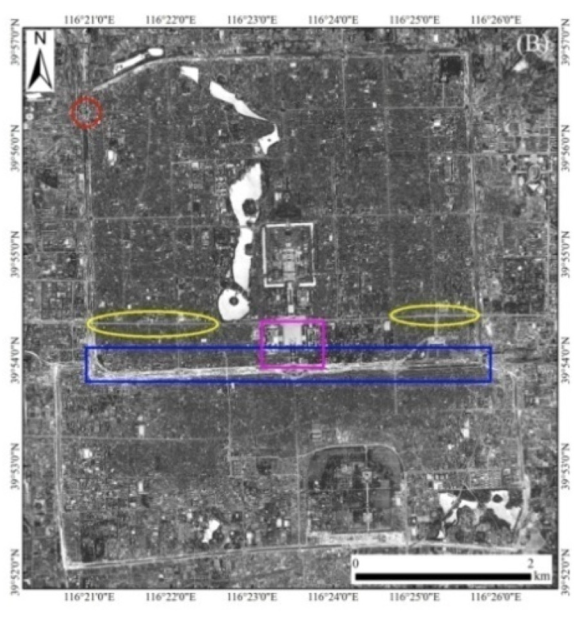
\includegraphics[height=7cm]{images/foto.png}
\caption{Aerial photograph in 1945 of Beijing \cite{asmr}}
\end{figure}

\subsection{Hyperspectral and multispectral image}
Unlike photography, which uses only frequencies within the visible range, hyperspectral and multispectral imaging uses a wider range of frequencies that are not visible to the naked eye.


Multispectral has wavelengths usually between the visible and infrared and typically uses 3 to 15 bands with a length greater than 20 nm. An example of the use of multispectral imagery is the Landsat-8 satellite, which produces 11 images from different bands, all but 3 of which have a resolution of 30 meters.

The following images show the different bands used in Landsat-8 imagery.

\begin{figure}[H]
\centering
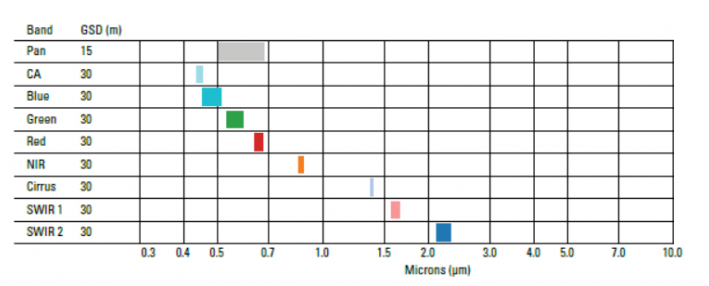
\includegraphics[width=10cm]{images/landsat1.png}
\caption{Landsat-8 bands from the OLI sensor\cite{landsat}}
\end{figure}

\begin{figure}[H]
\centering
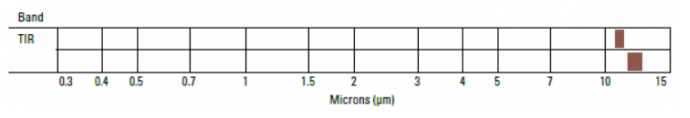
\includegraphics[width=10cm]{images/landsat2.png}
\caption{Landsat-8 bands from the TIRS sensor\cite{landsat}}
\end{figure}

Hyperspectral imaging, on the other hand, typically uses hundreds or thousands of narrower bands (typically smaller than 20nm).

These fundamental differences between multispectral and hyperspectral imaging have a major impact on archaeological prospecting, since the more and narrower the bands, the greater the ability to detect subtly different spectral reflections in the ground.

It is also worth mentioning that buried archaeological objects can have their chemical, physical and biological properties altered, causing differences in spectral reflectance.


\subsection{LiDAR}
LiDAR has become an essential part of archaeological prospecting. By attaching it to a drone, for example, it is possible to cover large areas in order to discover new sites with archaeological potential.  Its operation is based on emitting high-frequency light beams and then measuring the time it takes for the light beam to reach the object and return.
By analyzing the characteristics of the returned signal, it is possible to create a 3D map of the area in question.

The following image shows an example of a point cloud from an area in Viana do Castelo.

\begin{figure}[H]
\centering
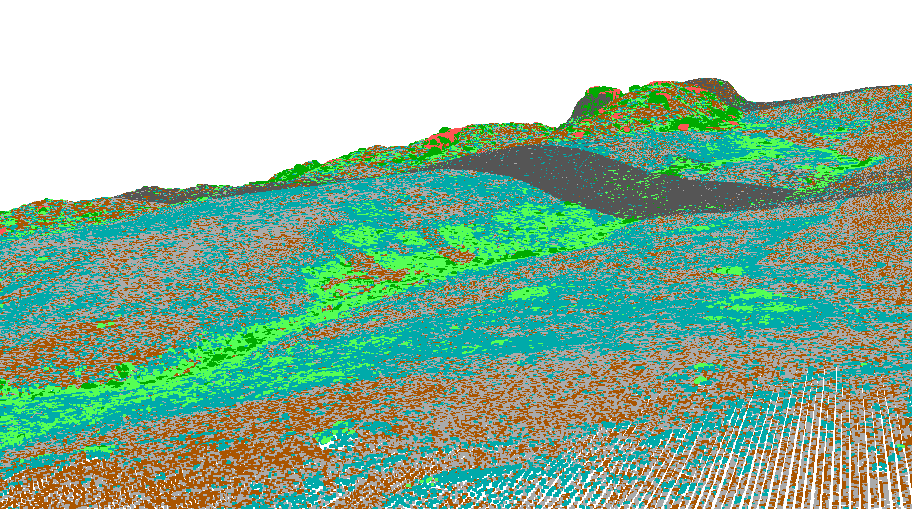
\includegraphics[width=10cm]{images/pointcloudViana.png}
\caption{Point cloud from Viana do Castelo}
\end{figure}

In the image each color of the point represents the category the point belongs to - for example green represents vegetation and brown represents soil.

As a result of the work of archaeologists and specialists, airborne lidar has been successfully used to detect archaeological features around the world. However, in order to be useful, it is first necessary to classify and fit the points in the point cloud, which is a crucial process to identify and remove points that do not belong to the ground in order to be able to detect archaeological features. The result of this filtering is called a \ac{dtm}. However, it should be noted that this method is not perfect and it is possible to filter too much, in this case filtering points that belong to archaeological objects.

The next image shows the same zone but filtered showing only the points classified as soil.
\begin{figure}[H]
\centering
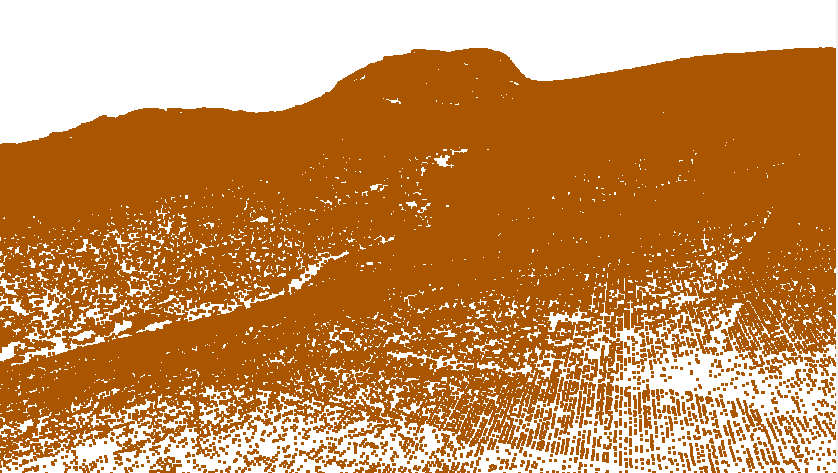
\includegraphics[width=10cm]{images/pointcloudVianafiltrado.png}
\caption{Point cloud from Viana do Castelo filtered}
\end{figure}

\section{Relief Visualization Techniques}

For the implementation of deep learning algorithms, one of the possibilities is to use directly the filtered Lidar radar data, i.e. to use the \ac{dtm}, as it is shown in the article \cite{deeplearningRawLidarData}. However, deep learning methods may have certain limitations, as many human resources are needed to make the annotations. In the case of archaeological annotations, if done by non-professionals, they may contain errors due to lack of knowledge of the scene and structure of the object in question. 

Another option is to pre-process the point cloud to create an image with the relief information. There are several techniques to create such images. In the article\cite{reliefModel} 13 methods are listed. However, we will only discuss the two most effective according to the article, e2MSTP and MSTP, and the LRM used in the thesis.

\subsection{MSTP and Enhanced MSTP}
One of the most efficient techniques used is \ac{mstp}. As explained in the \cite{mstp} article, it works well for visual interpretation and semi-automatic feature detection. By focusing on the topographical context of the structures rather than the structures themselves, it is particularly good for heterogeneous objects. Enhanced MSTP adds a morphological visualization technique to MSTP, creating a more detailed image.

The following image shows an MSTP image, a morphological visualization, and the result of combining the two, the enhanced MSTP image.

\begin{figure}[H]
\centering
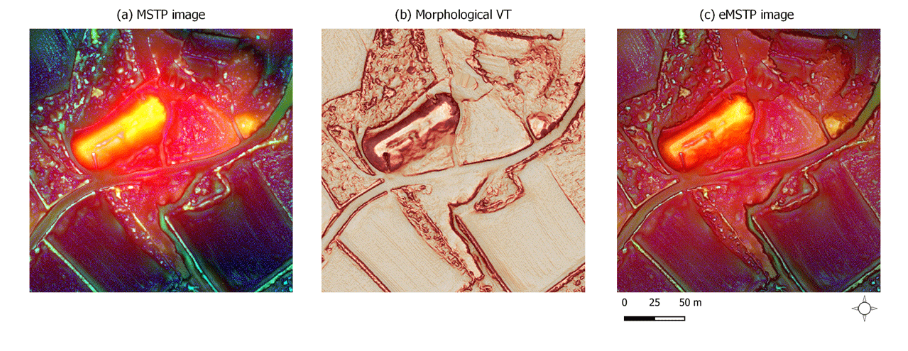
\includegraphics[width=12cm]{figs/mstp.png}
\caption{MSTP and Enhanced MSTP \cite{emstp}}
\end{figure}

It is important to note that this technique does not provide topographical measurements since the RGB values do not represent elevations or slopes.

According to \cite{emstp}, enhanced MSTP allowed researchers to obtain a detection accuracy of 77\%, proving thia to be a good technique especially if combined with the right deep learning model.

\subsection{Local relief model (LRM)}

Local Relief Model (LRM) is one of the most widely used techniques for archaeological purposes. In \ac{lrm} small-scale elevation differences are represented after the landscape is removed from the data, as in \ac{dtm}. 

The LRM significantly improves the detectability of shallow, small-scale topographic features, regardless of the lighting conditions. It enables direct measurement of both their relative heights and volumes\cite{lrm}.

When a low-pass filter is applied to the \ac{dtm}, it results in a smoothed elevation model, which serves as an initial representation of the large-scale landscape forms. The size of the kernel used in the low-pass filter determines the spatial scale of features captured in \ac{lrm}.

\section{Deep learning VS Machine Learning}

This section explains how it is possible to apply both deep learning and machine learning methods to archaeology.

Since LRM imaging is one of the most widely used techniques in archaeology, a logical next step is to apply deep learning methods to the detection of new archaeological sites. These methods can be objection detection or semantic segmentation. Both methods are based on CNN (Convolutional Neural Network).

\subsection{Convolution Neural Network }
\ac{cnn} is one of the most recurrent forms of deep learning because it is based on the human brain. Unlike classical machine learning, where it is necessary to first collect features from the dataset and then feed them into the machine learning algorithm, CNNs are also able to train filters that can extract these features.

The operation is based on an input layer, where the image passes through several convolution layers.
The convolution layer applies a set of filters or kernels to the input image, each of which extracts a specific feature from the image. For example, one filter might detect horizontal edges, another filter might detect vertical edges, and so on. The filter is moved over the input image, performing a point-to-point multiplication at each position, and the average of the sums of these multiplications is calculated to produce an output value at a given position. At the end, a feature map is created.

Between each convolution layer, it is normal to have a polling layer, which is used to reduce the size of the feature map to reduce the number of features. This layer divides the image into rectangular regions, and then for each region, simply takes the highest value or averages the values.
After the last max-poling layer come the dense layers, but for this you need to transform the image from matrix to vector, and for this a flatten layer is used.

The dense layers, also known as fully connected layers, are used to process the data from the previous layers.

Finally, we have the output layer, which can be a sigmoid if the result is binary, or a softmax if it is not.

\begin{figure}[H]
\centering
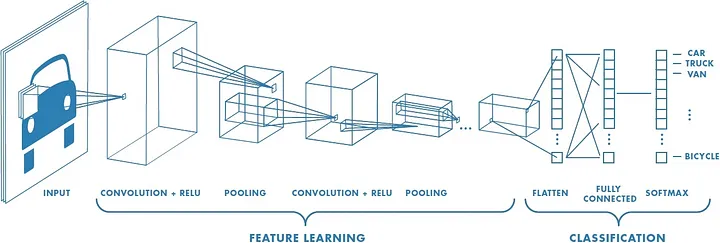
\includegraphics[width=15cm]{images/cnn.png}
\caption{Example of neural network \cite{mediumCNN}}
\end{figure}

\subsection{Machine Learning}
The main difference between deep learning and machine learning lies in the architecture and the level of complexity in the learned tasks. One notable distinction is the degree of human involvement. In deep learning, the model learns to extract features from the data on its own, while in traditional machine learning, humans need to manually extract features from the data and then provide them as input to the algorithm.

\begin{figure}[H]
\centering
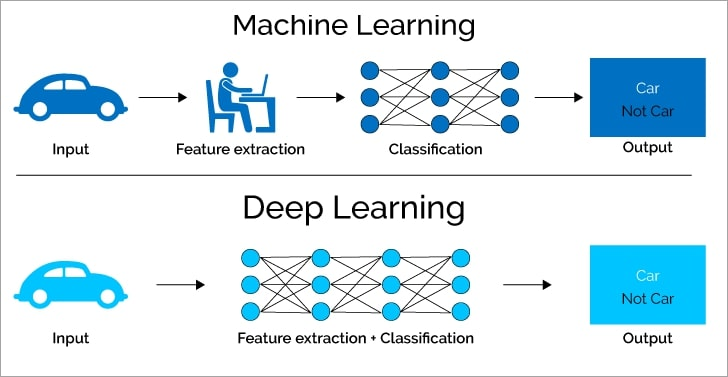
\includegraphics[width=15cm]{images/deepLearningVSmachineLearning.jpeg}
\caption{Machine Learning VS Deep learning\cite{deepLearningVSmachineLearning}}
\end{figure}

The use of machine learning methods in archaeology using the \ac{lidar} data without preprocessing is a technique that has been used. The unsupervised clustering based machine learning methods are more suitable for irregular object\cite{rawLidarjoaofonte}.

When it comes to cultural heritage, surface or structural defects often appear in the form of irregular geometric features. These can include weathering, cracks, and partial defects. As a result, these algorithms are exceptionally well suited for identifying and extracting surface defects in such cases.

\chapter{Dataset preparation}

\begin{introduction}
In this chapter, it will be discussed various ways of applying artificial intelligence models to archaeology.
\end{introduction}





Deep learning is a subtype of artificial intelligence, which relies on neural networks in order to recognize patterns in given training data. When trained on a dataset, the network is able to learn many features of the dataset, becoming able to make predictions when presented with new data.


%One of the pillars of deep learning is the diversity of the dataset, and also the precision of the training annotations, because the model will be able to learn small possible variations in the data, reducing the risk of overfitting, therefore a good dataset is fundamental, however it is not always possible to obtain a dataset that represents all the input possibilities.

%\subsubsection{Overfitting}
%Overffiting occurs when a model performs very well on training data, yet when presented with new data has difficulty making correct predictions. This can occur for several reasons:
%\begin{itemize}
%\item There is too little training data, creating a dataset that is unrepresentative of all possible inputs.
%
%\item The model is trained for a long time and thus, without stopping early, increasingly makes the model only an expert on the given type of training data.
%
%\item The model is too complex, causing it to learn not only the necessary predictive features, but also the noise that the inputs may have.
%\end{itemize}

To perform the Odyssey project, the Alto Minho region, Portugal, was chosen. With the help of the Comunidade Intermunicipal do Alto Minho, LiDAR data of 2018 was collected, covering 2220 km2, being later applied the visualization technique, more specifically LRM. As a result of this process 4 LRM images were generated, corresponding to 4 sub-regions of Alto Minho: Viana do Castelo, Paredes de Coura, Arcos de Valdevez and Parque Nacional da Peneda-Gêrez, with each pixel corresponding to 0.5 meters on the terrain.
From these 4 sub-regions, the locations of all known tumuli and castros were also noted.

The following table shows the resolution of each image, as well as the number of known annotations and the image size.

\begin{table}[h!]
\centering
\begin{tabular}{|p{3cm}|p{2.5cm}|p{2cm}|p{2cm}|p{2cm}|} 
 \hline
  Region & Resolution(px) & Annotations (tumulis) & Annotations (hillforts) & Size (GB) \\ [0.5ex] 
 \hline\hline
 Viana do Castelo & 19,978x46.000 & 14 & 41 & 3.7\\ 
 Paredes de Coura & 13,999x51,999 & 56 & 65 & 2.9 \\
 Arcos de Valdevez & 15,999x43,999 & 71 & 46 & 2.8\\
 Parque Nacional da Peneda-Gerês & 19,999x44,955 & 135 & 11 & 3.6\\ [1ex] 
 \hline
\end{tabular}
\caption{Description of the dataset used}
\end{table}

The following image shows the joint of the 4 LRM images, corresponding to the entire Alto Minho area where LiDAR data was collected.

\begin{figure}[H]
\centering
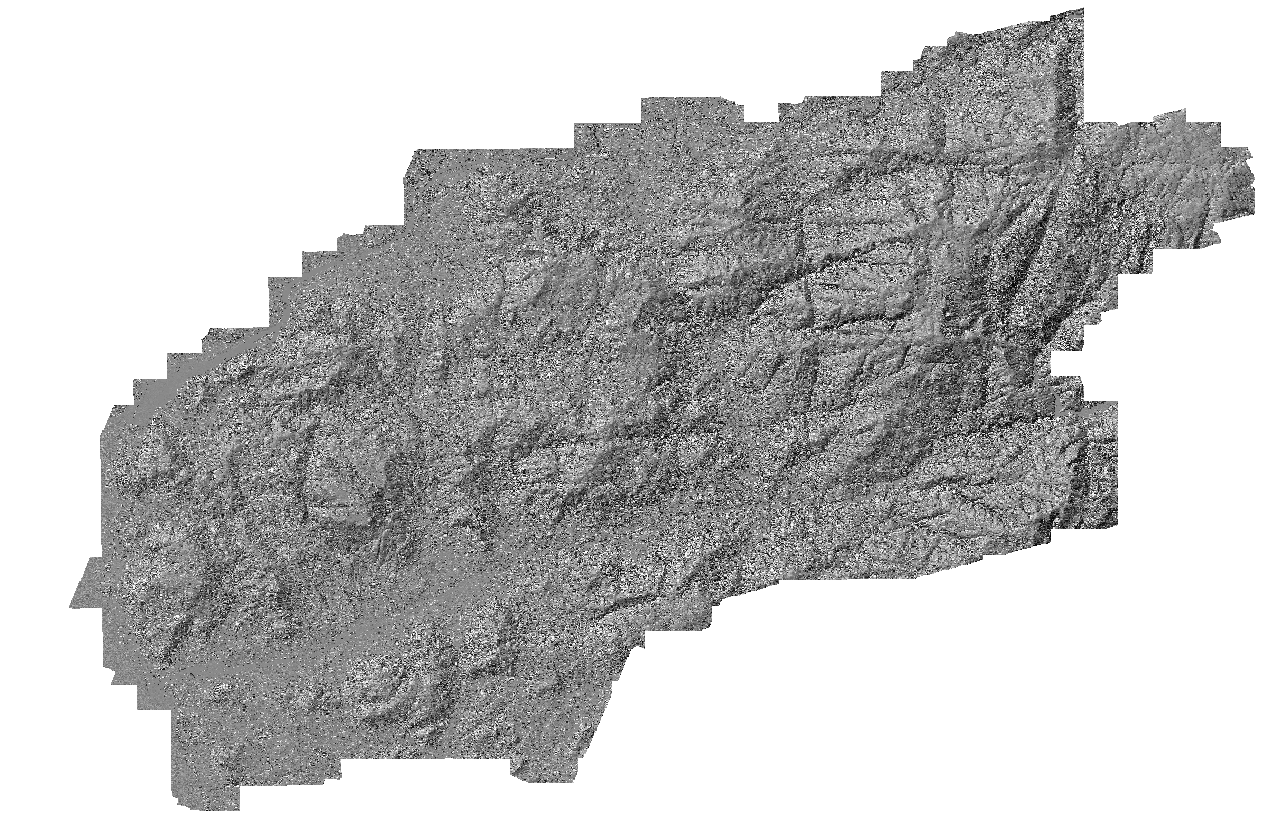
\includegraphics[width=10cm]{images/LRMfinal.png}
\caption{The 4 LRM images together, corresponding to Alto Minho}
\end{figure}





%That said, in this project the amount of data provided is relatively small \cite{yolov5recomedacoes}, as you can see, it is recommended to use for each type of object more than 1500 images and more than 10000 annotations to have good results, and since YOLOv7 is a relatively large model, this is even more important, due to the possibility of the weights not converge all if the dataset is small, and that is what this section is about, creation of the dataset, as well its augmentation.

\subsection{Creation of the base dataset}

With the LRM images, the locations of known tumuli and hillforts were provided in the Well-Know Text (WKT) format. This format indicates in polynomial form the geographical location of the site in question.

However, as it is possible to see from the table above, the 4 LRM images are too large, both for training the YOLOv7 model and the Unet model. Because of this, the 4 images were processed in order to obtain a dataset with 640x640 pixels images, being a typical size to train both YOLOv7 and Unet.

For this, a Python script was used. In this script, one LRM image was loaded at a time, as well as its annotations. To simplify it, separate datasets were generated for the tumuli and for the forts. Then, the annotations were parsed, and using the LRM image metadata, the geographic coordinates of the image extremities were obtained. With that, the coordinates present in the annotation polynomials were converted to pixels using the mapping function, as illustrated below:

\begin{equation}
     pixel = \frac{(coordenate - inMin) * (outMax - outMin)} {(inMax - inMin)} + outMin
     \label{Map function}
\end{equation}

In the function, the inMin and inMax represent the geographic coordinates of the LRM image extremities, whereas the outMin and outMax represent the size of the image in pixels. However, in the y-coordinate, are counted from top to bottom. Therefore, to calculate the y-coordinate of the pixel, outMin and outMax are swapped.


As previously stated, 4 LRM images have been provided as well as the annotations of where the archaeological sites are located. In order to generate the dataset, a python script was used. From the 276 tumuli provided, 161 images were generated, each image containing between 1 and 9 tumuli, for the hillforts 150 images were created, containing 152 sites, each image containing between 1 and 2 hillforts. With the same script, .las files were also generated, for each annotation, each file only contains the points of the cloud of points corresponding to the object in question, this files will be later use to train a machine model, with the objective to validate the results from the YOLOv7. Note that the annotations in the YOLOv7 format, follow the following format, annotation type, center point (x, y), width and height, both the center point and the measures are normalized.

Initially the annotations were transformed from GIS reference to pixels and then into boundind boxes, because the provided annotations came segmented, i.e. in the form of polygons as shown in the figure below.

\begin{figure}[H]
\centering
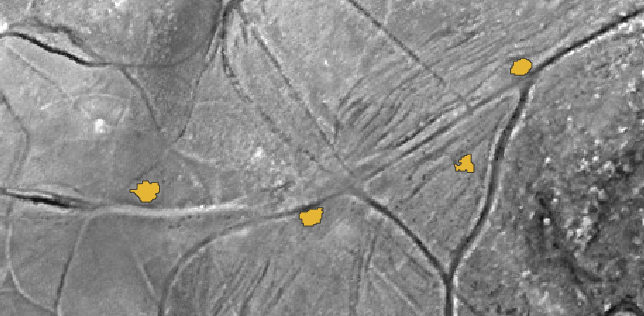
\includegraphics[width=10cm]{images/segmentacao_mamoas.png}
\caption{Original annotations}
\end{figure}
It is worth to mention that each pixel corresponds to 0.5 meters in the ground.

After that, for each bounding box not yet processed, the script randomizes a position for the object inside a 640x640 pixel image, if all objects are completely inside the image, the image is generated as well as its labels.

As can be seen, the number of annotations are far from the ideal, so two algorithms were used to generate an augmented datasets.

\subsection{Augmentation copy paste}

The first augmentation algorithm, which I will refer to as copy-paste augmentation.

The copy paste algorithm consists in copying objects (tumuli or hillforts) to other areas, creating a larger dataset.

For this algorithm, a deep learning model, YOLOv5, was trained with only the initial data, and a topographic chart of the area under study was also used. 

Initially it was performed the cropping of the annotations with the segmentation, having the objects cropped was applied one of the following geometric transformations, flip left to right, flip top to bottom, rotate 90, 180 or 270 degrees and transpose.
Once this is done, random areas were selected where there are no annotations, which were then passed on the trained model only with the original dataset, to make sure that there are no undetected objects in that area. 

After this the object is pasted and to be sure that the image is not pasted on top of buildings, houses, rivers, roads, etc (areas where there would never be an object to detect), a topographic map of the area under study (Viana do Castelo) is used in order to check if the randomly selected zone can be chosen. At the end the final 640x640 pixels images are generated together with the text files containing the labels.

\begin{figure}[H]
\centering
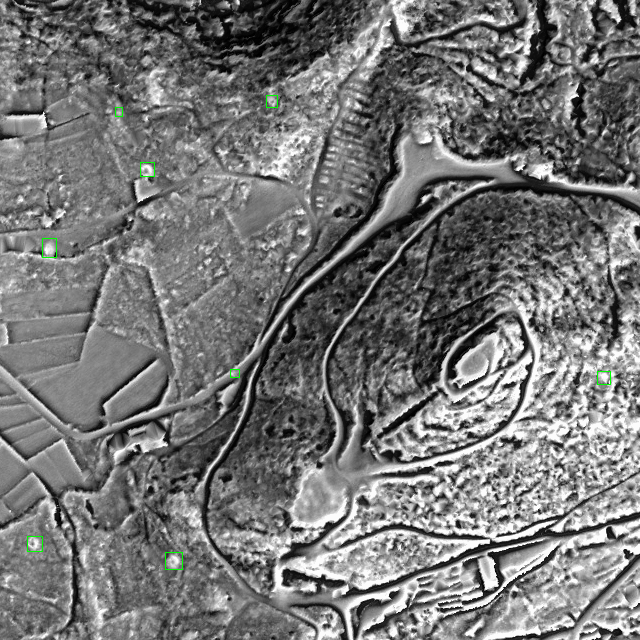
\includegraphics[height=9cm]{images/mamoas_aug_example.png}
\caption{Example of copy paste augmentation}
\end{figure}

\subsection{Simple augmentation}
The second augmentation algorithm, which will be called simple augmentation, which as the name indicates, is much simpler than the first one, this one is based on centering each object in a 640x640 pixels box and moving the box randomly, after that verify if the object is completely inside the box, as well as other nearby objects, if all the objects are inside the box, one of the same transformations of the previous algorithm is applied, but not to the object itself but to the image, finally the images are saved as well as the labels

This way it is possible to have the same annotation but in a different position of the image, with different backgrounds.

\subsection{Augmentation results}

Analyzing the github repository which contains the code needed to run YOLOv7, is possible to verify that no recommendations for creating a custom dataset are indicated, not even in the published paper \cite{paperyolov7}, in which it is only indicated that the COCO dataset was used to train the model and nothing else is mentioned about datasets. 

However in the YOLOv5 repository, there is a section, where it is given recommendations on how to train a custom dataset, and as said before, it is recommended per object type to have more than 1500 images and more than 10000 annotations \cite{yolov5recomedacoes}.

Following this recommendation for the copy paste increase, a dataset was generated for the 2754 images containing a total of 18398 tummies, noteworthy that within these 2754, 130 are from the original dataset.

For the simple augmentation, not as many as recommended were used, 1380 images were generated, with a total of 3124 tummies.

For the hillforts, with copy paste augmentation, 2464 images were generated, with a total of 6925, also here the 140 images are from the original dataset. Here the number of castros was reduced a little, not reaching the recommended 10000, due to their size, usually large objects, the image would be too populated and unrealistic.

For the simple augmentation 815 images were generated with a total of 844 hillforts.

FALTA AQUI alterar o numero dos castros que estao mal



\chapter{Object detection}

\begin{introduction}
In this chapter we will present one of the techniques used to detect archaeological sites, object detection.
\end{introduction}

One of the challenges of artificial intelligence is image classification, i.e. identifying which class the content of the image belongs to. However, another more challenging problem is object detection, i.e. identifying where the object is within the image.

One of the first algorithms to be made for this purpose, is the RCNN, this algorithm consists in generating about 2000 regions of interest in the image with the selective search algorithm, and then make image classification in these 2000 proposed regions, using a CNN. Although this algorithm can give good results, one of the problems is that it is very slow, giving an average of 47 seconds per image. 

Later, two other algorithms were created, the Fast RCNN and the Faster RCNN, showing improvements, the latter being able to process an image in mere seconds.

Later in 2016, a paper was published of a model, with an architecture called You Only Look Once (YOLO), which has since had several versions, the latest being YOLOv8.
YOLO is considered state of the art when it comes to object detection.

Of the methods presented in the previous chapter, the one chosen was the image creation from the information provided by the LIDAR, and 4 LRM images were created. However the creation of these images is not part of this dissertation, having been provided by another group belonging to the ODYSSEY project, as well the annotations.

Having the LRM images and the respective annotations, the objective of this chapter is to use YOLOv7 to discover archaeological sites.

Esta parte nao esta muito bem!!!!!!!!!!!!!!!!!!!!!!!!!!

The annotations are provided as csv files, however each annotation is saved in WKT (Well-known text) format.

The objects of study will be tumuli and hillforts, there are a total of 270 tumuli and 163 hillforts, however these annotations are not the result of a deep analysis of the terrain, thus creating the possibility that there are more objects
to detect.

After creating the dataset, the YOLOv7 model was trained, as well as a
machine learning model, with the raw data, in an attempt to eliminate false positives resulting from YOLOv7.

The two objects under study, are quite different, the tumuli on the one hand, have a very regular shape, uniform and of very equal size, on the other hand, the hillforts already have a very non-uniform shape and various sizes.

Finally, the training results of the trained models will be analyzed.


\section{YOLO}
While the 3 methods presented, RCNN, Fast RCNN, and Faster RCNN, all of them run the image several times through the algorithm, YOLO comes with a different idea, the image only passes through the model once.

For this, the image is divided into a grid with several cells, the image is then processed by the model, generating a two dimensional tensor, with the number of rows equal to the number of cells, and columns equal to 5 + number of object classes. In other words, each cell has a vector associated with the probability of having an object with the central point of the bounding box inside it.

y = [pc, cx, cy, w, h, c0, c1, c2,...].

\begin{itemize}
    \item pc is the probability of being the identified object.
    \item cx and cy is the center point of the bounding box.
    \item w and h are the width and height of the bounding box.
    \item c0, c1, c2, ... indicates which class the detection belongs to.
\end{itemize}

However, this approach presents a problem, because for the same object several bounding boxes can appear, for this the algorithm uses a function called NMS (Non Maximum Suppression).

\subsubsection{Non Maximum Suppression}
Non Maximum Suppression \cite{nonmaxsurpression} is a method that selects a region from a series of overlapping regions. First it discards all proposed regions with a probability below a certain threshold. For the remaining ones it chooses the region with the highest probability and discards all the others that have an IoU higher than a certain threshold.
IoU is the intersection over union, that is the area of the region in question divided by the union of the areas of all the regions that overlap with that same region.

IoU is the intersection over union, this means the area of intersection of the overlapping regions to be divided by the area of the union.


\subsection{Training}
Neural network training is a fundamental step in deep learning, it is in this phase that the network will "learn" how to perform the task at hand, this can range from image classification, object detection, language processing and many other applications.

To do this it is common to divide the dataset into 3 parts, training, validation and testing. During training the net goes through several iterations called epochs, where it learns to make predictions by adjusting its internal parameters based on the provided training data.
The training process consists of feeding the neural net with batches of training data.
A batch is a subset of the training data set, instead of feeding the entire training data set to the neural net, it is divided into batches, making the process more computationally efficient, and also allowing the weights of the neural net to be adjusted more often, since they are updated at the end of each batch.

At the end of the batch processing, the error is calculated relative to the predictions made by the model and the labels. This error is usually measured by a loss function, such as cross entropy or least squares error. After the error is calculated, the optimization algorithm, such as SGD or Adam, is used to adjust the weights of the neural network in a direction that minimizes the error. To do this a back propagation function is used, where the error is propagated from the output layer to the input layer, allowing each neuron to update its weights in order to contribute to the reduction of the total error.

At the end of each epoch, a validation of the model is then performed with the validation set, that is, the data from the validation set is used to evaluate the performance of the trained model up to that point. Model validation is crucial for monitoring the generalization ability of the model over the course of training. It provides information on how the model is performing on data not used during training, and helps identify problems such as overfitting. Overfitting occurs when the model overfits on training data, losing the ability to generalize to other input data.

It is at this stage that the hyperparameters, values that control the learning process, are updated, one of them being for example the learning rate.
At the end of training, inference is performed on the test set, which consists of data never before seen by the model. While the validation set is used to adjust the hyperparameters and is thus indirectly seen during training, the test set remains completely unknown to the model until that moment.

\subsubsection{Pre-trained models}
One of the techniques widely used in deep learning is the use of pre-trained models, especially when the available dataset is relatively small. 

The main advantage of pre-trained models is that they capture knowledge and patterns learned from massive datasets, which can be applied to specific tasks with smaller datasets. They are able to extract relevant features and abstract representations from the input data, which makes them more effective in the task at hand.

Although unpre-trained models have almost the same accuracy as unpre-trained models, the robustness and uncertainty of the model change dramatically, as can be seen in the article \cite{pretrainedmodels}.

This means that for new input data, never before seen by the model, the model can make better predictions as well as be more certain of the results, giving a higher probability of the results.



\subsubsection{YOLOv7 training}
In order to train the model, all the generated datasets were divided into training and validation data, 85\% training and 15\% validation. The test dataset was not used, because, at the end of training, an inference was performed on the original LRM images.

For the number of epochs, several values were chosen, varying between 200 and 350, and for the batch the largest allowed by the project's computer hardware was chosen, a batch of size 8.

\subsubsection{Cross fold validation}
A technique that is also widely used is cross fold validation, which is known to offer good results, especially when the dataset is small. This technique consists in splitting the total dataset into K folds, and then using each fold as validation data and the others as training, generating K models.

This method is useful, because the whole available dataset is used to train K - 1 models, which makes it possible to analyze whether there are significant differences in the use of different parts of the dataset.

This technique has only been used on the dataset generated with copy paste augmentation on tummies. The dataset was divided into 5 folds, each fold containing 550 images.



\subsection{Training results}

YOLOv7 already provides the python script needed for training and also saves the training results. These training results are fundamental to understand if the model was well trained or not. Several metrics are used for this, some of them being the confusion matrix, accuracy, mAP and F1.

The confusion matrix is nothing more than a table with the values of true positives, false positives, true negatives and false negatives (TN). True positives (TP) are all predictions generated by the model where an object actually exists, false positives (FP) are predictions where the object in question does not exist, true negatives (TN) are predictions where the model is all the background given by the model, which actually corresponds to background and finally, false negatives are all objects that were not detected by the model.

Accuracy is the ratio between all correct predictions and all predictions generated by the model, given by the following formula:

\begin{equation}
     Accuracy = \frac{TP + TN}{TP + TN + FP + FN}
\end{equation}
Two other values that can be obtained are accuracy and recall\cite{https://towardsdatascience.com/on-object-detection-metrics-with-worked-example-216f173ed31e}. Precision refers to what percentage of the predictions made are true positives,in other words, how accurate is the model in identifying only relevant objects, and is given by the following formula:

\begin{equation}
     Precision = \frac{TP }{TP + FP}
\end{equation}

Recall on the other hand tells us the ability of the model to identify ground truths and is given by the following formula:

\begin{equation}
     Recall = \frac{TP }{TP + FN}
\end{equation}

To obtain the graph of both precision and recall, several confidence values are used, i.e. the value that is required to be trusted for each detected object, so that it is not discarded. As a rule, a higher confidence value leads to a higher recall, while a lower confidence value leads to a higher precision. Taking the precision and recall values in pair for several confidence values, the graph recall vs precision is generated, being the area under the curve the corresponding AP (Average precision). To calculate if a detected object is a false positive or not, a function called IoU (intersection over union) is used.

For a detected object to be considered a true positive, it is necessary that the area of intersection between the bounding box of the detected object and the bounding box of the ground truth divided by the union of the two areas is greater than a certain threshold. When this value is 50\%, the AP is called AP50.

\begin{equation}
     IoU = \frac{\text{Intersection area}}{\text{Union area}}
\end{equation}

\begin{figure}[H]
\centering
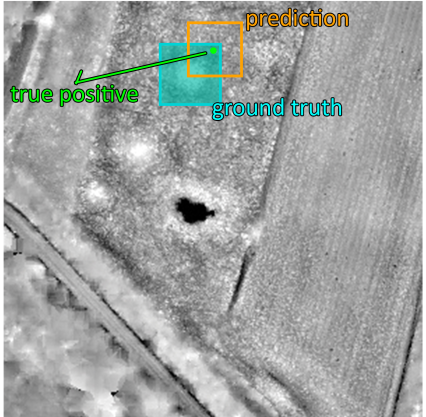
\includegraphics[height=8cm]{images/IOU.png}
\caption{Example of IoU \cite{Deep Learning for Archaeological Object Detection on LiDAR:
New Evaluation Measures and Insights}}
\end{figure}

Having the APs of all classes, the mAP is then calculated by taking the average of the APs, however in this project separate models were trained for each class, making the AP equal to the mAP.

Another metric is F1, which is given by the following formula:

\begin{equation}
     F1 = 2 * \frac{precision * recall}{precision + recall}
\end{equation}

This metric is especially interesting, when both accuracy and recall are important, enabling an analysis of which is the most favorable confidence value.

Another metric that is also commonly used, is mAP0.5:0.95, the difference with mAP50, is that instead of using only a minimum value of IoU to consider a true positive, several values between 50\% and 95\% are used, with 5\% jumps.

When it comes to lof, training data is unavailable. Additionally, unlike yolo, the original dataset cannot be expanded due to its raw lidar data nature. Given the limited size of the dataset, all the generated .las files were utilized and as mentioned in \cite{lof}, performing inference on training data can yield inaccurate outcomes.

\subsection{Training results}
In this subsection the training results of yolov7 will be shown. Training was performed with all the generated datasets, which are 4 for the tummies and 3 for the hillforts.

As said before the dataset was divided in 85\% for training and 15\% for validation, no test set was used, since the original dataset provided was small, and also because an inference will be made on the LRM images, so it will be possible to analyze the model's performance, analyzing if it found all the annotated objects as well as new ones.

First the training results for the tumuli will be analyzed, and then the results for the hillforts will be analyzed.

In the case of yolov7 training with the original dataset the result was as shown below:

\begin{figure}[H]
    \centering
    {{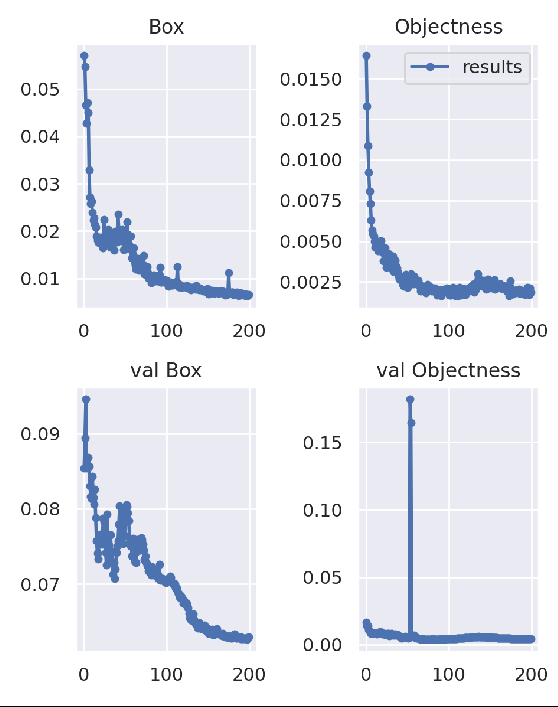
\includegraphics[width=5cm]{images/training/mamoas/notaug1.png} }}
    \qquad
    {{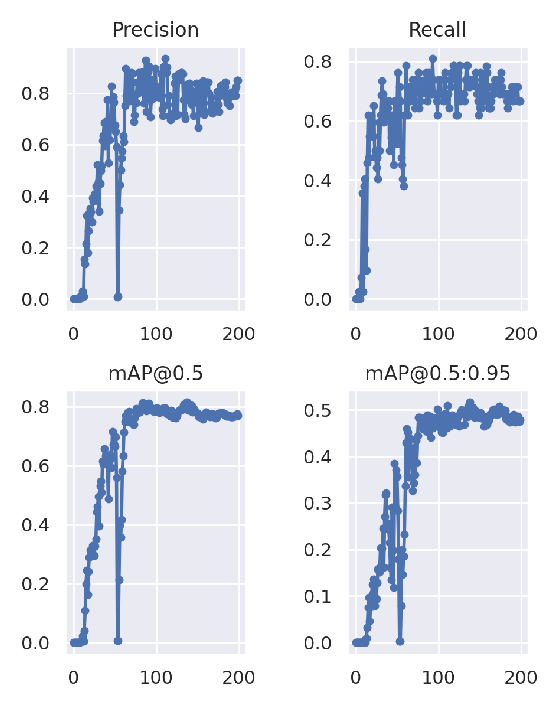
\includegraphics[width=5cm]{images/training/mamoas/notaug2.png} }}
    \caption{Results of Yolov7 training with tumulis non augmented dataset}
    \label{fig:example}
\end{figure}

In the case of training with the dataset augmented with the copy paste algorithm the result was as shown below:

\begin{figure}[H]
    \centering
    {{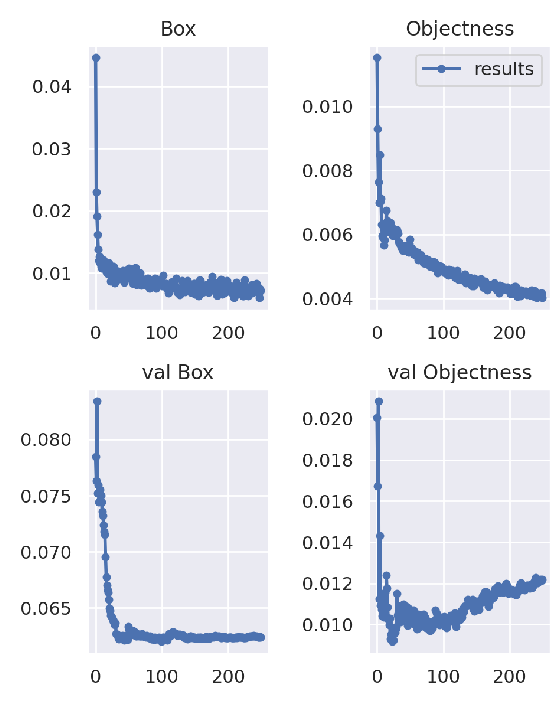
\includegraphics[width=5cm]{images/training/mamoas/aug1.png} }}
    \qquad
  {{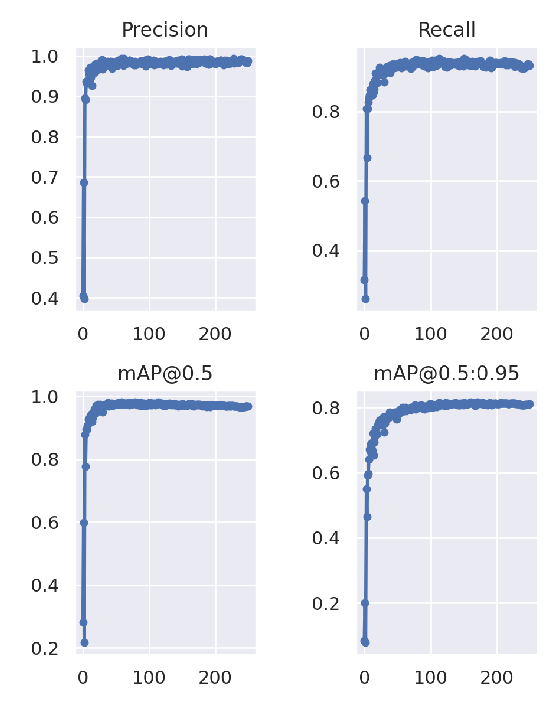
\includegraphics[width=5cm]{images/training/mamoas/aug2.png} }}
    \caption{Results of Yolov7 training with tumulis augmented dataset (copy paste)}
    \label{fig:example}
\end{figure}

In the case of training with the dataset augmented with the simple algorithm the result was as shown below:

\begin{figure}[H]
    \centering
    {{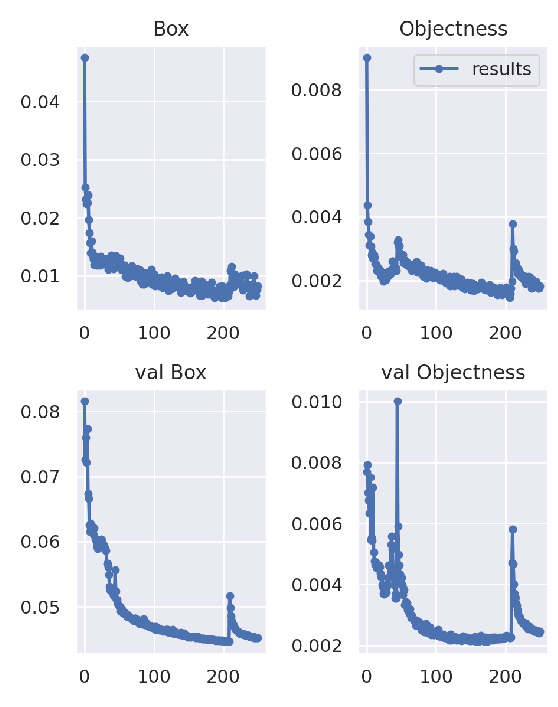
\includegraphics[width=5cm]{images/training/mamoas/maia1.png} }}
    \qquad
    {{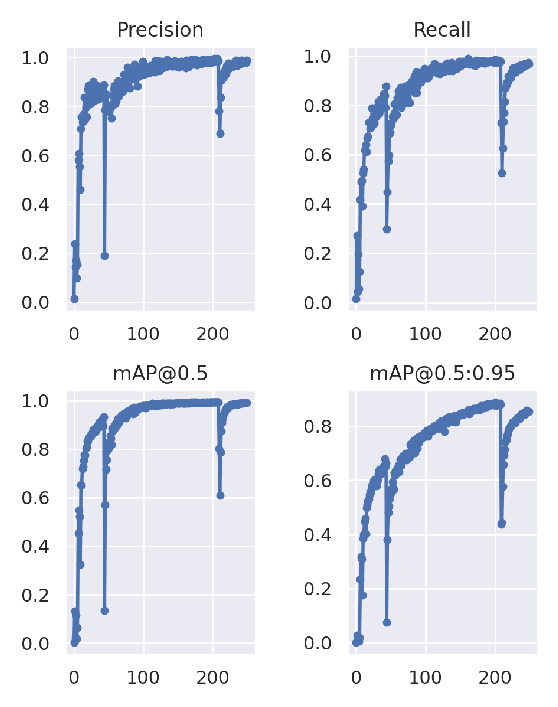
\includegraphics[width=5cm]{images/training/mamoas/maia2.png} }}
    \caption{Results of Yolov7 training with tumulis augmented dataset (simple)}
    \label{fig:example}
\end{figure}

In order to analyze these results, my focus will be solely on the mAP0.5 metric rather than the F1 score. The reason behind this choice is that mAP provides a consolidated value that combines both precision and recall for each epoch, while F1 score represents a graph for each epoch, making it a more complex metric to work with.

As can be observed, in neither of the three models did overfitting occur, including training with the dataset not augmented, which is the most prone to overfitting. It is interesting to note that in the copy paste dataset, after a few seasons, the model stabilized and got very close to 1.

Falta agora para o cross validation!!!!!!
Isso sera uma tarefa nao para o Leonardo de hoje mas sim para o Leonardo do futuro!

In the case of hillforts, the results are as follows:

\begin{figure}[H]
    \centering
    {{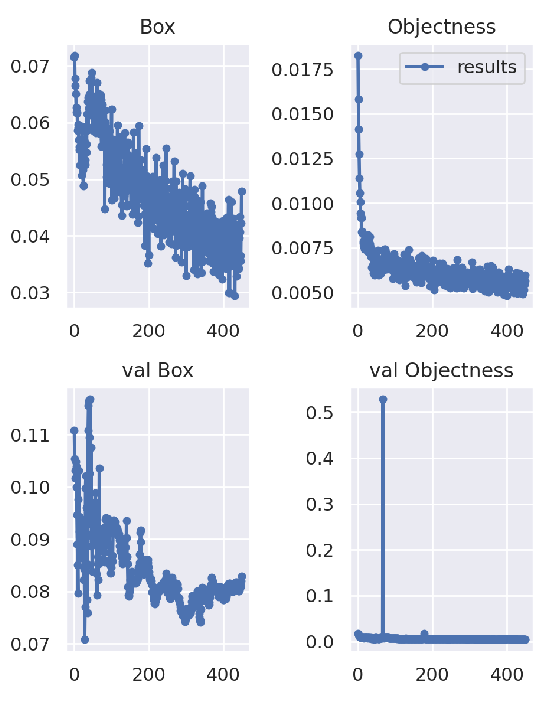
\includegraphics[width=5cm]{images/training/castros/notaug1.png} }}
    \qquad
    {{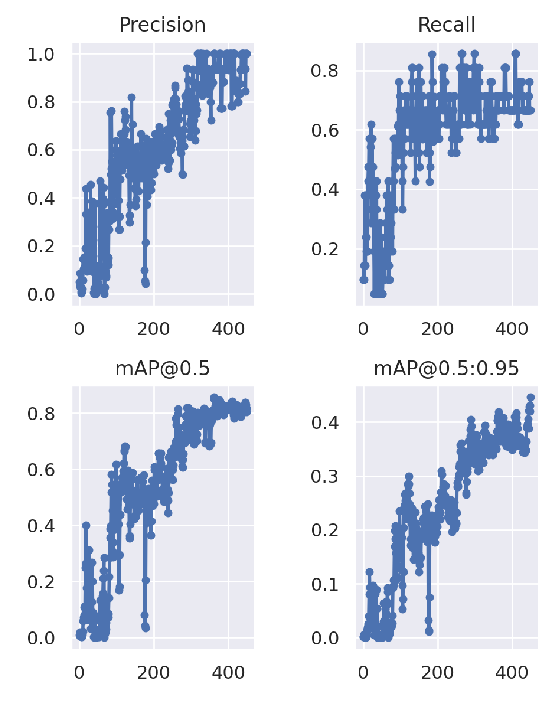
\includegraphics[width=5cm]{images/training/castros/notaug2.png} }}
    \caption{Results of Yolov7 training with hillforts non augmented dataset}
    \label{fig:example}
\end{figure}

In the case of training with the dataset augmented with the copy paste algorithm the result was as shown below:

\begin{figure}[H]
    \centering
    {{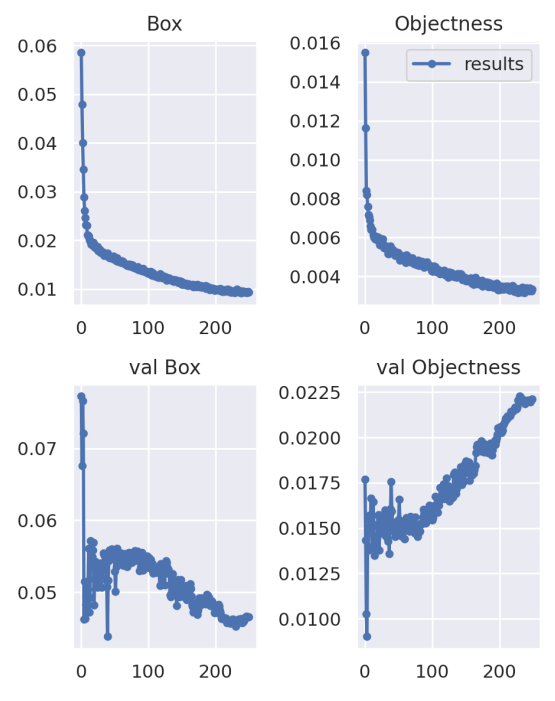
\includegraphics[width=5cm]{images/training/castros/aug1.png} }}
    \qquad
  {{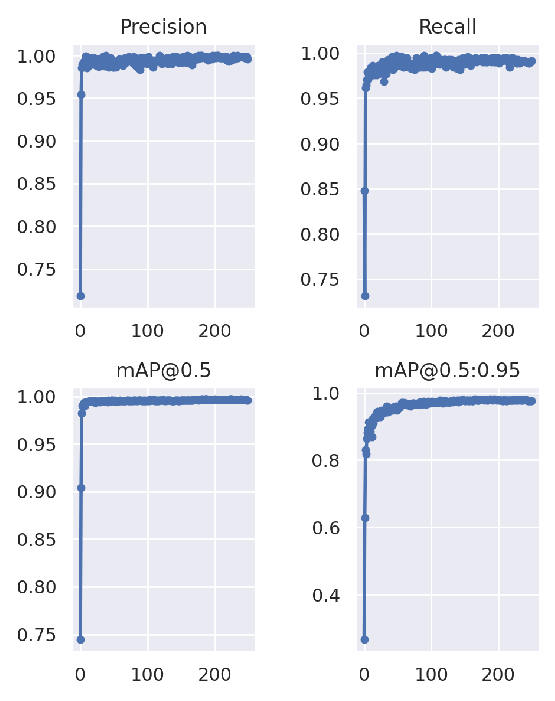
\includegraphics[width=5cm]{images/training/castros/aug2.png} }}
    \caption{Results of Yolov7 training with hillforts augmented dataset (copy paste)}
    \label{fig:example}
\end{figure}

In the case of training with the dataset augmented with the simple algorithm the result was as shown below:

\begin{figure}[H]
    \centering
    {{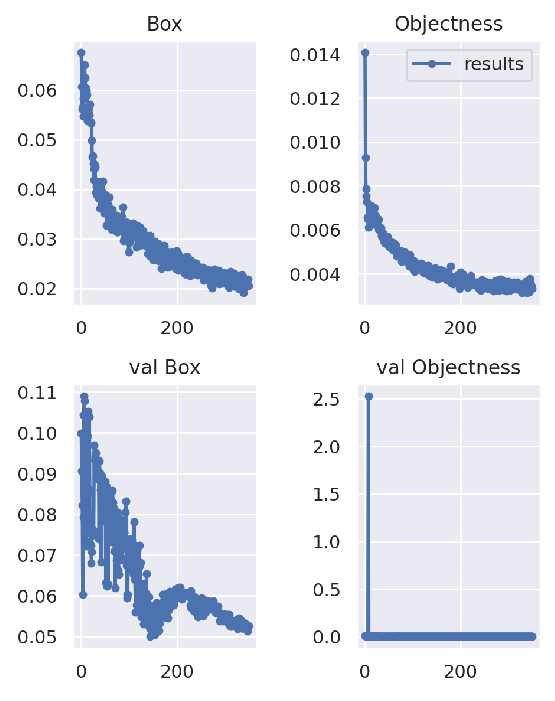
\includegraphics[width=5cm]{images/training/castros/maia1.png} }}
    \qquad
    {{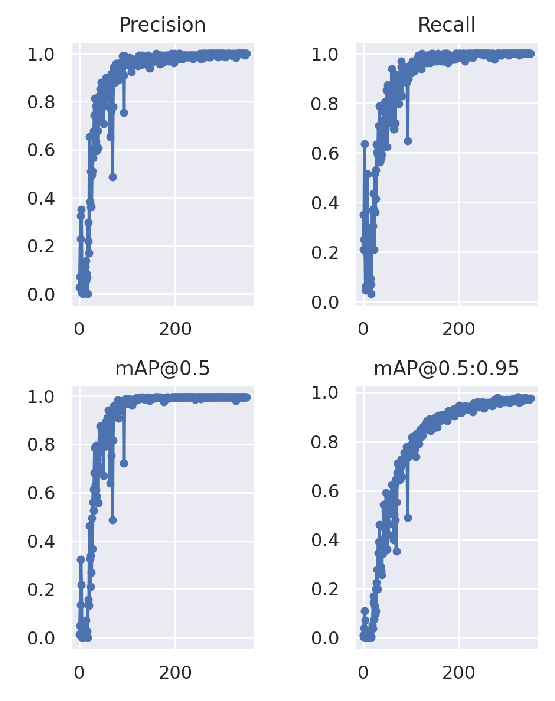
\includegraphics[width=5cm]{images/training/castros/maia2.png} }}
    \caption{Results of Yolov7 training with hillforts augmented dataset (simple)}
    \label{fig:example}
\end{figure}

Similarly to the tummy tucks, in none of the three workouts, overfitting occurred. In the case of the training with the unenhanced dataset, it was necessary to increase the number of seasons in order to make the model converge. And similarly to the tumuli training, the hillforts training with the copy paste dataset, after a few seasons, the mAP was already close to 1.

\subsection{Inference}
In this subsection we will show how the inference was done on the 4 LRM images.

In order to do the inference, a python script was created, in this script, the image is loaded with the PIL library and then, the geographic coordinates of the 4 corners of the image are obtained using the rasterio library, this is possible because the tif images can contain additional information such as geographic coordinates. 

Having the coordinates, and the images being too large to make inferences, an interactive window was used, in order to perform 640x640 pixel crops, however this approach leads to a problem, the crop can be done on top of an object, leaving a part of the object in one image and another part in the next image, to work around this a sliding window was used instead of a fixed window, with the sliding window instead of cropping in a fixed way at each position, the image is scrolled in a systematic way by moving the window pixel by pixel or at a defined interval. This approach allows each object or region of the image to be covered by multiple inference windows, thus avoiding the problem of having parts of an object split between different crops.

When using the sliding window, the image is divided into overlapping windows that move along the image. Each sliding window captures a specific region of the image and then inference is applied to that region individually. As the window slides, new regions are processed, ensuring that all objects or regions are covered.

For the tumuli a 50\% slide was used, because they are small objects, and for the hillforts a 30\% slide was used, because some hillforts occupy almost half of the cropped image.

Once the crop is obtained, it is checked with the aid of a topographic chart to see if the crop contains areas that are likely to have objects. This means that in the crop, there are areas where, for example, there are no houses or roads, thus discarding crops that represent, for example, a residential area in its entirety. After that, inference is performed with YOLO. As mentioned before, YOLO can make multiple detections for the same object, so to overcome this, the NMS function is also used here, discarding overlaps and all inferences with a confidence lower than 25\%. Then, once again, the topographic chart is used to verify if the object is not in an area where it would be impossible to detect.

Once the inference is completed, the identified objects undergo validation using the LOF model. To validate each object, a temporary LAS file is generated. This file is created by utilizing the geographical coordinates of the bounding box. The temporary LAS file is then populated with points that fall within the bounding box. Next, various statistical measures such as mean, median, variance, standard deviation, and covariance are computed using the 14 features extracted from each point. Finally, a prediction is made, returning a value of 1 if the object is determined to be a true positive, or 0 if it is classified as a false negative.

Finally, due to the window slide, for the same object there may be several inferences, because when making the slide the same object may still appear in the next image. To mitigate this, initially the Euclidean distance was used, all the bounding boxes that had the center less than 15 pixels, which corresponds to 7.5 meters on the ground, from another one, would be removed. Initially this approach worked well for the tumuli. However, for the hillforts, a problem occurred, the yolo was detecting hillforts inside larger hillforts, something that does not happen in reality, making it difficult to choose a threshold value for the Euclidean distance. 

In order to get around this, the Euclidean distance was replaced by IoU, as explained before, if the IoU was smaller than a certain value, the smaller hill was discarded, however, the problem still remains, as I checked later in article \cite{Deep Learning for Archaeological Object Detection on LiDAR}, if the smaller hillfort is fully contained in the larger one and if the area of the smaller one is smaller than the defined threshold value, IoU does not discard, so the problem still remains. So the approach was adopted, instead of being the normal IoU the intersection. Therefore, instead of using the normal IoU, the intersection to be divided by the union, the division of the intersection to be divided by the area of the smallest detection was used. But before that the objects were ordered by area, from the biggest to the smallest, by doing that and using this modified version of the IoU, in the cases where there are detections completely contained inside another, or almost completely contained, they are removed, keeping the biggest one.

In the end, the results are saved in a csv file, containing the geographic coordinates of the bounding box, the confidence given by yolo and the result of the LOF validation.

After the completion of the inference, it is necessary to assess the efficacy of the model by analyzing the detected ground truths and new objects. To facilitate this analysis, a Python script has been developed. Within this script, the ground truth coordinates are loaded and converted into corresponding image pixels, which are further transformed into bounding boxes. Similarly, the coordinates of the objects resulting from the inferences are processed. Utilizing the Shapely library, both the ground truth objects and the inferred objects are converted into polygons. Subsequently, a filtering process is applied to the inference results, removing any inferences with an area smaller than 90\% of the smallest ground truth area. Finally, an interaction is performed on the ground truth objects to determine which inference results intersect with the ground truth.

In the case of inference with the 5 models generated from cross validation, YOLOv7 provides a technique called model ensemble, in which it is allowed to use several models at the same time.

\subsubsection{Model ensemble}
Model ensemble is a technique that consists in using predictions from several deep learning models in order to obtain more robust results than a single model could provide.

By using several models trained on different datasets, in this case the cross validation models, each model generates its own predictions. After that, the predictions are combined, for this, techniques such as majority voting, weighted average, probability average, among others, being possible to make a final decision.

The idea behind this is that each model can capture different features or aspects of the training dataset, and by combining these various models, it is possible to compensate the failures of one model by the successes of others, thus making the result more reliable.

\subsection{LOF model training}
One of the problems encountered earlier in the dissertation was that the inference results contained many false positives, in an attempt to solve this problem, a Local Outlier Model (LOF) was trained on the raw LIDAR data.

Using the .las files generated during creation of the dataset, containing only the points within the bounding box surrounding the object in question, two LOF modelsm, one for tumulis and one for hillforts, were trained using the scikit learn library\cite{lof}.

LOF calculates the local outlier factor for each sample in the data set, taking into account the local density of neighboring samples. It compares the density of the sample against the average density of its nearest neighbors. If the density of the sample is significantly lower than the average density of its neighbors, this indicates that the sample is a possible outlier.

\begin{figure}[H]
\centering
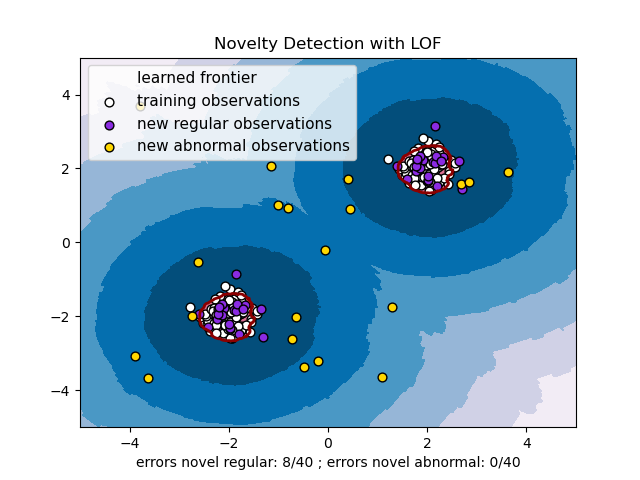
\includegraphics[]{images/lof_example.png}
\caption{Example of clusters generated by LOF}
\end{figure}

In order to train the model, jakteristics library was used, this library allows 14 features to be taken from each point in the point cloud, these features are: eigenvalue sum, omnivariance, eigenentropy, anisotropy, planarity, linearity, PCA1, PCA2, surface variation, sphericity, verticality, nx, ny and nz.

As each point contributed 14 features, this results in a huge amount of features, the mean, median, variance, standard deviation and covariance are calculated, resulting in an amount of 70 features per .las file.

\subsection{Inference results}
In this sub-section we will show the results of the inferences made on the 4 LRM images.

Tables will be presented, in which will appear the total number of detected objects, within these objects the number of validations made by the LOF, as well as the true positives, false positives and false negatives, the last 3 are in relation to the total number of detected objects and not to the ones validated by the LOF.

\begin{table}[h!]
\centering
\begin{tabular}{|c c c c c|} 
 \hline
  & Non augmented  & Copy Paste & Simple & Cross Validation(Copy paste) \\ [0.5ex] 
 \hline\hline
 Total & 2324 & 2366 & 1800 & 11446 \\ 
 Validations & 1604 & 1500 & 1354 & 6385 \\
 True positives & 240 & 224 & 210 & 242 \\
 False positives & 2084 & 2142 & 1590 & 11204 \\
 False negatives & 36 & 52 & 66 & 34 \\ [1ex] 
 \hline
\end{tabular}
\caption{Results of inference for tumulis}
\end{table}

\begin{table}[H]
\centering
\begin{tabular}{|c c c c|} 
 \hline
  & Non augmented  & Copy Paste & Simple \\ [0.5ex] 
 \hline\hline
 Total & 8002 & 1913 & 5630 \\ 
 Validations & 2799 & 628 & 2145\\
 True positives & 153 & 153 & 113 \\
 False positives & 7849 & 1760 & 5517 \\
 False negatives & 10 & 10 & 50\\ [1ex] 
 \hline
\end{tabular}
\caption{Results of inference for hillforts}
\end{table}
It is important to emphasize that the false positives and true positives are relative to the available ground truth, i.e. the training and validation data, and as said before, these data are not the result of an intensive terrain analysis, and there may be among the false positives that are in fact true positives, i.e. new sites discovered by the algorithm that have not yet been annotated.

However, according to the company that provided the data, most of the sites were noted, with only a few missing that may have been missed.

Analyzing the data resulting from the inferences, we can verify that there were many false positives, both in the tumuli and in the castros, however, in the tumuli, the worst case was the one resulting from cross validation, giving about 7 times more false positives than the model resulting from simple augmentation, on the other hand, it was the one that had fewer false negatives, that is, it was the one that managed to detect more ground truth.

In the case of the castros, the model that gave fewer positive false was the one resulting from the copy paste augmentation, giving 1750 negative false and detecting almost all the ground truths, failing only 10 in 163.


\chapter{Conclusions and Future Work}
\label{chapter:conclusion}

\begin{introduction}
This section highlights the insights gained from the analysis of the work that is currently being developed on the topic of this dissertation, as well as how the existing solutions will support the construction of this dissertation's work
\end{introduction}

The development of a lifelog retrieval system is a complex undertaking that requires effective collaboration across various modules that address different tasks. This dissertation aims to extend a module of the MEMORIA lifelogging system by implementing different image annotation algorithms to extract relevant information from image lifelogs. Because these collected annotations will be used by other components of the system, they must be structured and optimised to provide information in a valuable way. This can be accomplished by selecting the optimal models for this particular use case.

There are numerous solutions that are currently being developed in order to advance the state of the art in various computer vision tasks that meet the aims of this work. An investigation of a part of these solutions was carried out, allowing for the exploration of potential models to be included in MEMORIA's pipeline. 

These potential models were chosen considering what type of annotations are intended to be extracted from the lifelog images. It was defined that each image should be analysed on different levels of detail, which means that lower-level annotations such as the identification of objects and optical characters should be allied to higher-level ones such as the understanding of the scene depicted in the image as well as the identification of the global meaning of the lifelog.

This completed research process serves as a starting point for the next phase of the work plan, in which each prospective model will be tested in an isolated environment to see whether it is a suitable candidate for inclusion in the retrieval system. After testing each model, they will be integrated in the system and their performance will be analysed. It is expected that the integration of these new models will result in a solution that will allow effective lifelog retrieval utilising information derived from lifelogs images submitted to the MEMORIA system.







\chapter{Conclusions and Future Work}
\label{chapter:conclusion}

\begin{introduction}
This section highlights the insights gained from the analysis of the work that is currently being developed on the topic of this dissertation, as well as how the existing solutions will support the construction of this dissertation's work
\end{introduction}

The development of a lifelog retrieval system is a complex undertaking that requires effective collaboration across various modules that address different tasks. This dissertation aims to extend a module of the MEMORIA lifelogging system by implementing different image annotation algorithms to extract relevant information from image lifelogs. Because these collected annotations will be used by other components of the system, they must be structured and optimised to provide information in a valuable way. This can be accomplished by selecting the optimal models for this particular use case.

There are numerous solutions that are currently being developed in order to advance the state of the art in various computer vision tasks that meet the aims of this work. An investigation of a part of these solutions was carried out, allowing for the exploration of potential models to be included in MEMORIA's pipeline. 

These potential models were chosen considering what type of annotations are intended to be extracted from the lifelog images. It was defined that each image should be analysed on different levels of detail, which means that lower-level annotations such as the identification of objects and optical characters should be allied to higher-level ones such as the understanding of the scene depicted in the image as well as the identification of the global meaning of the lifelog.

This completed research process serves as a starting point for the next phase of the work plan, in which each prospective model will be tested in an isolated environment to see whether it is a suitable candidate for inclusion in the retrieval system. After testing each model, they will be integrated in the system and their performance will be analysed. It is expected that the integration of these new models will result in a solution that will allow effective lifelog retrieval utilising information derived from lifelogs images submitted to the MEMORIA system.





%%%%%%%%%%%%%%%%%%%%%%%%%%%%%%%%%%%%%%%%%%%%%%%%%%%%%%%
% End of Thesis text 
%%%%%%%%%%%%%%%%%%%%%%%%%%%%%%%%%%%%%%%%%%%%%%%%%%%%%%%

\backmatter

%%%%%%%%%%%%%%%%%%%%%%%%%%%%%%%%%%%%%%%%%%%%%%%%%%%%%%%
% Print all used references
%%%%%%%%%%%%%%%%%%%%%%%%%%%%%%%%%%%%%%%%%%%%%%%%%%%%%%%

\begingroup
\renewcommand{\bibfont}{\footnotesize}
% Redefine References name to Portuguese
% Change if you are using english
\defbibheading{bibliography}[References]{
	\chapter{#1}
}
\SingleSpacing
\setlength\bibitemsep{8pt}
\printbibliography[heading=bibliography]
\endgroup


%%%%%%%%%%%%%%%%%%%%%%%%%%%%%%%%%%%%%%%%%%%%%%%%%%%%%%%
% Load appendix
%%%%%%%%%%%%%%%%%%%%%%%%%%%%%%%%%%%%%%%%%%%%%%%%%%%%%%%

%\include{appendix-a}
%\include{appendix-b}
%\include{appendix-c}

\end{document}
